\todo{Will fix the formatting once content is finalized.}
%%%%%%%%%%%%%%%%%%%%%%%%%%%%%%%%%%%%%%%%%%%%%%%%%%%%%%%%%%%%%%%%%%%%%%%%%%%%%%%%%%%%%
\section{Queries}
\label{app:queries}
%%%%%%%%%%%%%%%%%%%%%%%%%%%%%%%%%%%%%%%%%%%%%%%%%%%%%%%%%%%%%%%%%%%%%%%%%%%%%%%%%%%%%

\subsection{Kate's Restaurant Recommendation}

\subsubsection{SQL}

% Listing \ref{lst:sql1KateRest} works as follows: First, the reviews, user, and business tables are joined together to find out which businesses Kate reviewed. Once all these businesses are obtained, all users who rated these businesses above 3 stars are obtained by another review join. Finally, the categories table (and its linking table) is joined to the businesses to only include restaurants.

\lstinputlisting[
    language=sql,
    caption={
        A SQL query that returns ``recommending users'' of Kate (a user in the dataset). These are users who have reviewed restaurants that Kate has also been to with a rating above 3 stars.
    },
    label={lst:sql1KateRestAppen}
]{./queries/kate1.sql}

% Listing \ref{lst:sql2KateRest} begins by joining the review and business tables to match all businesses reviewed by the given user. These businesses are filtered by those within the Las Vegas area (with a radius of 50km). The reviews are ordered by date and limited to return only 10, as to keep only the latest reviews from the user.

\lstinputlisting[
    language=sql,
    caption={
        A SQL query that returns the star rating, text and business ID for restaurants a user has reviewed above 3 stars.
    },
    label={lst:sql2KateRestAppen}
]
{./queries/kate2.sql}


\subsubsection{Gremlin}

% The query in Listing \ref{lst:gremlin1KateRest} works by obtaining the vertex representing Kate and declaring the referencing for this vertex using the \texttt{as} step. The review edges leaving Kate are then filtered by those with a star rating above 3. The \texttt{inV()} step simply refers to the businesses who have the incoming review edge. The \texttt{in("REVIEWS")} step is different from the \texttt{inE} step as it skips across the edge and references the user vertices directly -- which are then selected if they are not Kate's vertex. These users are referenced and the category vertices are checked to filter out businesses which aren't restaurants. The users referenced earlier are then selected, duplicates are removed and their ID values are selected for the return.

\lstinputlisting[
    language=gremlin,
    caption={
        A Gremlin query that returns ``recommending users'' of Kate (a user in the dataset). These are users who have reviewed restaurants that Kate has also been to with a rating above 3 stars.
    },
    label={lst:gremlin1KateRestAppen}
]
{./queries/kate1.groovy}

% Listing \ref{lst:gremlin2KateRest} starts again at the user vertex. The reviews are once again filtered by rating and then ordered by date. The reviews are then referenced for later twice as this can be used to create a dictionary-style output later. The vertices with these incoming review edges are implicitly business vertices again and are selected by their location using the mixed spatial index from ElasticSearch. These businesses are referenced for later. The reviews are selected and limited to 10 and all the prior references are selected. The dictionary-style output is produced using a combination of the \texttt{select} and \texttt{by} step\footnote{\texttt{select} will select the prior references and the \texttt{by} step will select the attribute to display from the references in \texttt{select} respectively.}. The output will now look like a list of dictionary objects with the keys; \texttt{stars}, \texttt{text}, and \texttt{business\_id} which are easily serialized and deserialized over sockets or a REST API.

\lstinputlisting[
    language=gremlin,
    caption={
        A Gremlin query that returns the star rating, text and business ID for restaurants a user has reviewed above 3 stars.
    },
    label={lst:gremlin2KateResAppent}
]
{./queries/kate2.groovy}

\subsubsection{GSQL}

% GSQL queries work by first declaring variables and seeds, then writing the query. The GSQL query in Listing \ref{lst:gsql1KateRest} declares a \texttt{SetAccum} which does not allow duplicates and the three seeds; \texttt{categories}, \texttt{businesses}, and \texttt{PSet}. First, businesses which are categorized as restaurants are selected, then businesses which were rated by the user -- which will be Kate. The users who reviewed the intersection of these two business sets are then accumulated based on the constraints that their ratings were above 3 stars and that those users aren't Kate. The results of the accumulated users is then printed which returns a JSON string of the variable's contents when the REST endpoint is queried.

\lstinputlisting[
    language=gsql,
    caption={
       A GSQL query that returns ``recommending users'' of Kate (a user in the dataset). These are users who have reviewed restaurants that Kate has also been to with a rating above 3 stars.
    },
    label={lst:gsql1KateRestAppen}
]
{./queries/kate1.gsql}

% Listing \ref{lst:gsql2KateRest} begins by declaring a custom type which has a tuple format. This allows one to record only the properties one wants to, similar to the \texttt{select} and \texttt{by} steps in Listing \ref{lst:gremlin1KateRest}. A \texttt{HeapAccum} is constructed with a max size of 1000, and is used as it can order the accumulator by the properties in the custom type -- in this case the date property. Using the geo-grid, all grid IDs are obtained using the \texttt{getNearbyGridId} method, which is then converted into a vertex set by matching the grid IDs to their respective vertices in the graph. The businesses connected to these grid vertices is obtained and businesses categorized as restaurants are then intersected as before Listing \ref{lst:gsql1KateRest}. The top 10 tuples from the heap are popped and accumulated in a list which is then printed.

\lstinputlisting[
    language=gsql,
    caption={
        A GSQL query that returns the star rating, text and business ID for restaurants a user has reviewed above 3 stars.
    },
    label={lst:gsql2KateRestAppen}
]
{./queries/kate2.gsql}

\subsection{Review Trends in Phoenix 2018}

\subsubsection{SQL}

% This kernel is the least complex of the three as it has a single join with a spatio-temporal constraint. Listing \ref{lst:sqlReviews2018} returns selected characteristics on reviews where the date year is 2018 and reviewed businesses are within the Phoenix area.

\lstinputlisting[
    language=sql,
    caption={
        A SQL query that returns all the review text and ratings for businesses within 50km of the Phoenix area during 2018.
    },
    label={lst:sqlReviews2018Appen}
]
{./queries/reviews.sql}

\subsubsection{Gremlin}

% One caveat of using mixed indexes on dates via the Gremlin Translator is highlighted in the query for this kernel. Usually, since Gremlin is designed to be embedded, one should make use of objects when appropriate. Since JanusGraph is being queried from Python\footnote{Where ideally, it would be within a JVM language which has access to the JanusGraph specific classes and functions, e.g. Groovy.}, with no support for mixed query specific parameters, date related parameters need to be parsed using static methods from the \texttt{Instant} class in Java. This can be seen in Listing \ref{lst:gremlinReviews2018} when filtering reviews by date. Alternatively, one could also use the \texttt{filter} step as is done in Listing \ref{lst:gremlinCity}.

% Out of the set of businesses within the Phoenix area and set of all the reviews in 2018, the businesses set would be the smaller of the two. This is important when using a dataflow language since the whole subset will be accumulated before moving to successive functions in the query. Due to this characteristic of Gremlin, businesses are accumulated before the reviews.

\lstinputlisting[
    language=gremlin,
    caption={
        A Gremlin query that returns all the review text and ratings for businesses within 50km of the Phoenix area during 2018.
    },
    label={lst:gremlinReviews2018Appen}
]
{./queries/reviews.groovy}

\subsubsection{GSQL}

% Since only selected characteristics of a review are desired, a tuple is created at the beginning of Listing \ref{lst:gsqlReviews2018}. The businesses within the Phoenix area are selected first, then reviews where the date part is 2018. The review tuples are accumulated into a \texttt{ListAccum}. 

\lstinputlisting[
    language=gsql,
    caption={
        A GSQL query that returns all the review text and ratings for businesses within 50km of the Phoenix area during 2018.
    },
    label={lst:gsqlReviews2018Appen}
]
{./queries/reviews.gsql}

\subsection{Ranking Las Vegas by Friends' Sentiment}

\subsubsection{SQL}

% Listing \ref{lst:sqlCity} begins by joining reviews and businesses before joining the two depths of friend relations. Julie's ID must be checked for at depth two as to only include mutual friends. Businesses are constrained by location and reviews by their month value under the date attribute. All reviews where the user ID matches the IDs of friends at depth 1 or 2 are selected and the text and star ratings of these reviews is returned.

\lstinputlisting[
    language=sql,
    caption={
        A SQL query that returns all the review text from reviews written by friends and mutual friends for businesses within 30km of the Las Vegas center.
    },
    label={lst:sqlCityAppen}
]
{./queries/city.sql}

\subsubsection{Gremlin}

% Starting with Julie's user vertex at the beginning of Listing \ref{lst:gremlinCity}, direct friends and mutual friends are accumulated as \texttt{f1} and \texttt{f2} respectively. First, duplicate users are removed, then any instance of Julie's vertex is removed from the union of these two accumulated groups of friends.

% Once the traversal needs to be filtered by the temporal aspect, the same issue of having to call multiple functions due to the caveat in Listing \ref{lst:gremlinReviews2018} is encountered. The month value is extracted from each of these dates and filtered by their month values accordingly and referenced for later use. These reviews are then constrained by the locations of the business vertices by which they are connected. These reviews are then selected and their text and star rating data returned.

\lstinputlisting[
    language=gremlin,
    caption={
        A Gremlin query that returns all the review text from reviews written by friends and mutual friends for businesses within 30km of the Las Vegas center.
    },
    label={lst:gremlinCityAppen}
]
{./queries/city.groovy}

\subsubsection{GSQL}

% In a similar fashion to the Gremlin variant, the users from both depths of the friend relations are aggregated before removing Julie's user vertex. The \texttt{SetAccum} is used so duplicate user vertices should not be an issue. The intersection of the nearby businesses and businesses reviewed by the accumulated friend users are then used to extract the review data. Another \texttt{SetAccum}, \texttt{@@reviews}, is used to extract the text and star rating data from each review, where the reviews are constrained by their month values. The accumulated review data in \texttt{@@reviews} is then returned.

\lstinputlisting[
    language=gsql,
    caption={
        A GSQL query that returns all the review text from reviews written by friends and mutual friends for businesses within 30km of the Las Vegas center.
    },
    label={lst:gsqlCityAppen}
]
{./queries/city.gsql}

%%%%%%%%%%%%%%%%%%%%%%%%%%%%%%%%%%%%%%%%%%%%%%%%%%%%%%%%%%%%%%%%%%%%%%%%%%%%%%%%%%%%%
\FloatBarrier
\section{Data Analysis}
\label{app:analysis}
%%%%%%%%%%%%%%%%%%%%%%%%%%%%%%%%%%%%%%%%%%%%%%%%%%%%%%%%%%%%%%%%%%%%%%%%%%%%%%%%%%%%%

\subsection{Kate's Restaurant Recommendation}
\begin{table}[h]
    \small
    \centering
    \caption{The result of analysis on the review data of recommended restaurants. Only results with 5 reviews or more are displayed.}
    \begin{tabular}{ |p{3.25cm}||p{1.78cm}|p{1.59cm}|}
        \hline
        \rowcolor{Gray}
        \multicolumn{3}{|c|}{Businesses in Phoenix 2018} \\
        \hline
        \rowcolor{LightGray}
        Name & Pos Sentiment & Star Average                 \\
        \hline
        Paco's Tacos \& Tequila     & 92.9825\%  & 4.5833 \\
        Oak Steakhouse Charlotte    & 100.0\%    & 5.0 \\
        The Cheesecake Factory      & 100.0\%    & 4.4615 \\
        Block \& Grinder            & 90.0\%     & 4.3333 \\
        Best Wok                    & 100.0\%    & 4.2 \\
        \hline
    \end{tabular}
    \label{tab:kateResult}
\end{table}

\subsection{Review Trends in Phoenix 2018}

\begin{figure}[h]
    \centering
    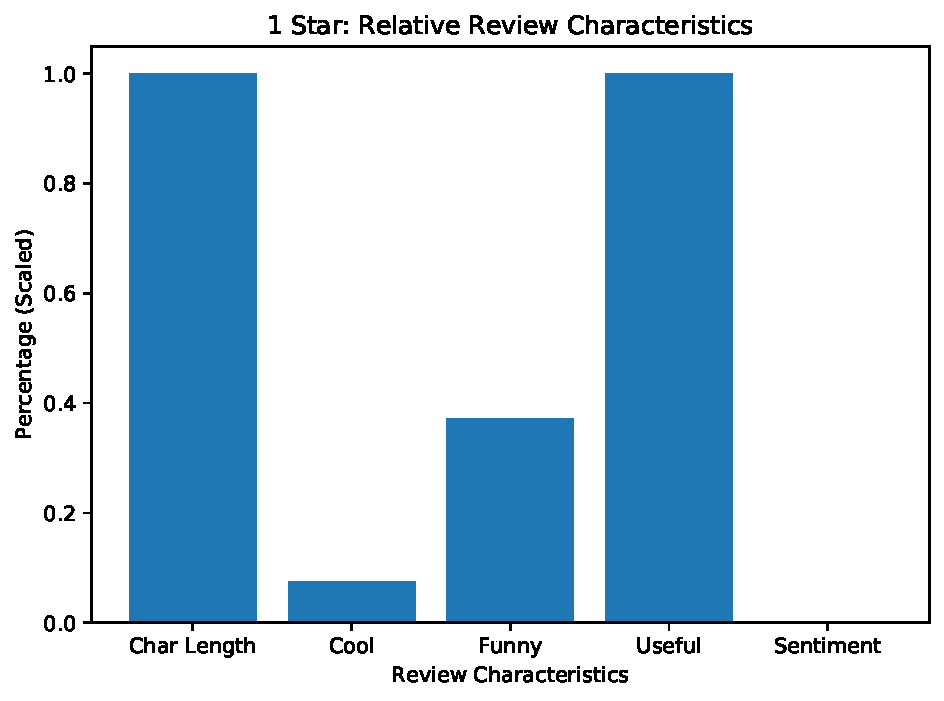
\includegraphics[width=0.49\textwidth]{img/phoenix2018/1Star.pdf}
    \caption{Relative characteristics of 1 star reviews over reviews of restaurants in Phoenix 2018.}
    \label{fig:1star}
\end{figure}

\begin{figure*}[h]
    \centering
    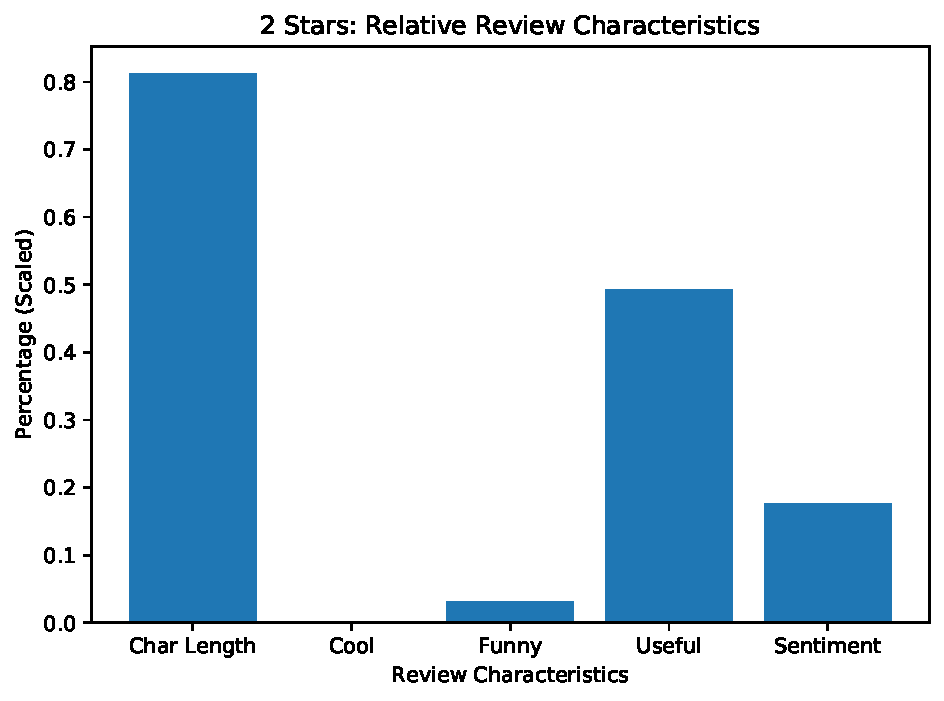
\includegraphics[width=0.49\textwidth]{img/phoenix2018/2Stars.pdf}
    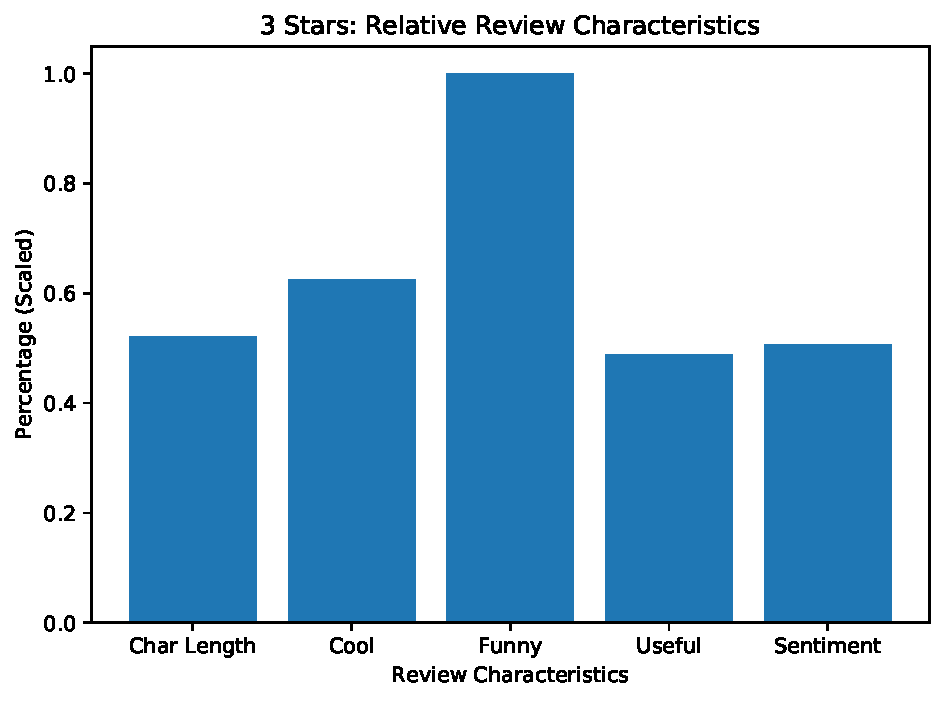
\includegraphics[width=0.49\textwidth]{img/phoenix2018/3Stars.pdf}
    \caption{Relative characteristics of 1 and 2 star reviews over reviews of restaurants in Phoenix 2018.}
    \label{fig:23star}
\end{figure*}

\begin{figure*}[h]
    \centering
    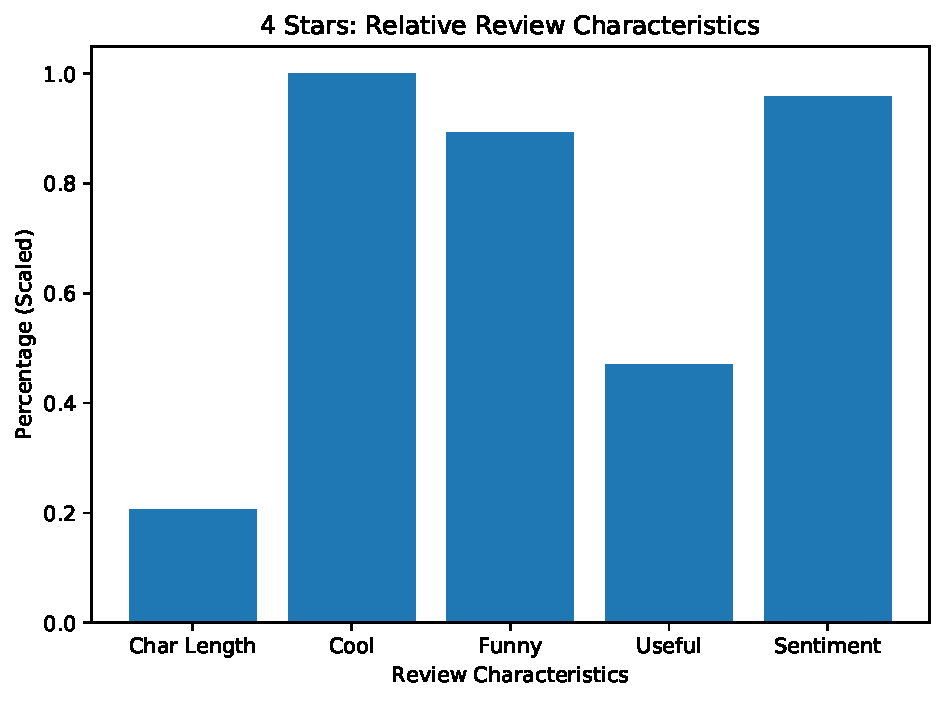
\includegraphics[width=0.49\textwidth]{img/phoenix2018/4Stars.pdf}
    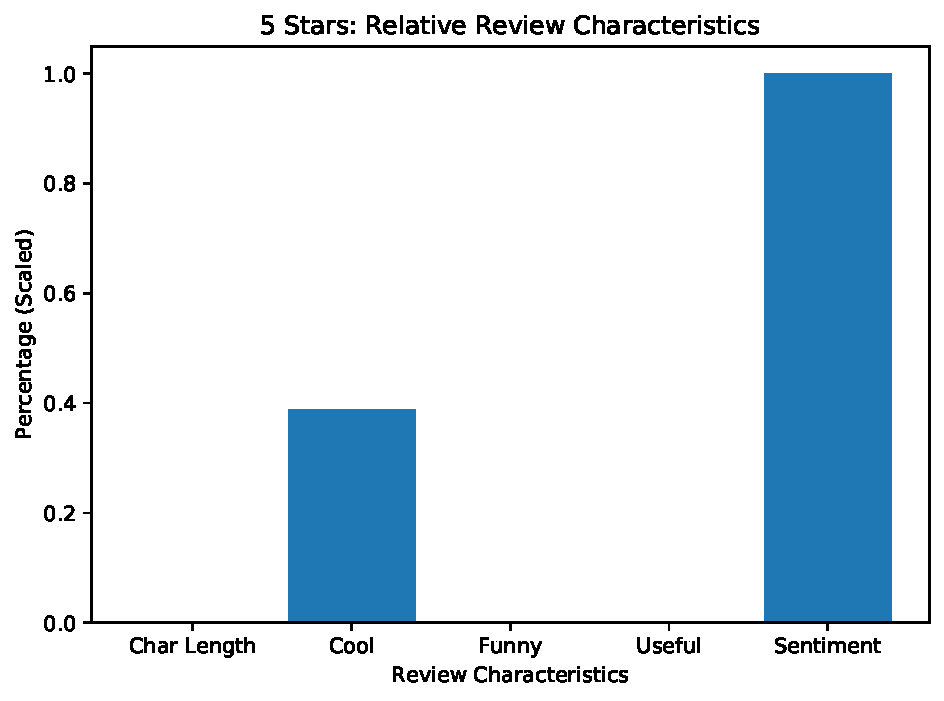
\includegraphics[width=0.49\textwidth]{img/phoenix2018/5Stars.pdf}
    \caption{Relative characteristics of 4 and 5 star reviews over reviews of restaurants in Phoenix 2018.}
    \label{fig:45star}
\end{figure*}

\FloatBarrier

\subsection{Ranking Las Vegas by Friends' Sentiment}

\begin{table}[ht]
    \small
    \centering
    \caption{The result of analysis on the review data of Julie's friends.}
    \begin{tabular}{ |p{3.5cm}|p{3.5cm}|}
        \hline
        \rowcolor{Gray}
        \multicolumn{2}{|c|}{Las Vegas Sentiment vs Star Average} \\
        \hline
        \rowcolor{LightGray}
        Positive Sentiment (\%) & Star Average \\
        \hline
        70.7767 & 3.8917 \\
        \hline
    \end{tabular}
    \label{tab:cityResult}
\end{table}